\documentclass{article}
\usepackage{graphicx}%
\usepackage{multirow}%
\usepackage{amsmath,amssymb,amsfonts}%
\usepackage{amsthm}%
\usepackage{mathrsfs}%
\usepackage[title]{appendix}%
\usepackage{xcolor}%
\usepackage{textcomp}%
\usepackage{manyfoot}%
\usepackage{booktabs}%
\usepackage{algorithm}%
\usepackage{algorithmicx}%
\usepackage{algpseudocode}%
\usepackage{listings}%




\usepackage{float}%make tables stay?



\providecommand{\keywords}[1]{\textbf{\textit{Keywords: ---}} #1}%keywords

\usepackage{parskip} %puts \noindent everywhere


\usepackage{caption}
\DeclareCaptionFormat{citation}{%
  \ifx\captioncitation\relax\relax\else
    \captioncitation\par
  \fi
  #1#2#3\par}
\newcommand*\setcaptioncitation[1]{\def\captioncitation{\textit{Source:}~#1}}%to add sources to figures
\let\captioncitation\relax
\captionsetup{format=citation,justification=centering}



%https://www.overleaf.com/project/642180d8a08db24a02633ac7


\usepackage{hyperref} 
% Hyperref setup
\hypersetup {
    colorlinks=true,
    urlcolor=blue
}

\usepackage{apacite}

\raggedbottom
%%\unnumbered% uncomment this for unnumbered level heads

\usepackage{geometry}
 \geometry{
 a4paper,
 total={170mm,257mm},
 left=20mm,
 top=20mm,

 }





\begin{document}

\title{\huge \scshape{Optimal TSP Solvers: Time-Constrained Algorithm Analysis}}
\author{
    \small \scshape{Harry Zhang} \\ 
    \small \scshape{Supervisors: Per-Olof Freerks and Felicia Dinnetz} \\
    \scriptsize \scshape{Kungsholmens Gymnasium}
}



\maketitle
\thispagestyle{empty} 
\newpage



\abstract{\noindent Gymnasiearbetet undersökte heuristiska algoritmer som löser det grafteoretiska handelsresandeproblemet. Algoritmerna testades på olika dataset med bestämd tidsbegränsning inriktad på att hitta den kortast möjliga rutten där alla angivna platser besökts.. The codes are available at \href{https://github.com/hairez/diploma-project}{https://github.com/hairez/diploma-project}.}

\keywords{travelling salesman problem, Euclidean distance, graph, Keyword4}

\thispagestyle{empty} 
\newpage

\abstract{\noindent The abstract serves both as a general introduction to the topic and as a brief, non-technical summary of the main results and their implications. Authors are advised to check the author instructions for the journal they are submitting to for word limits and if structural elements like subheadings, citations, or equations are permitted. The diploma project examined several heuristic algorithms designed to solve the travelling salesman problem within graph theory. The algorithms aimed to identify the shortest path covering all points within a predetermined time limit on various datasets. The codes are available at \href{https://github.com/hairez/diploma-project}{https://github.com/hairez/diploma-project}.}

\keywords{travelling salesman problem, Euclidean distance, graph, Keyword4}



\thispagestyle{empty} 
\newpage

\tableofcontents
\thispagestyle{empty} 
\newpage


\section{Introduction}\label{Introduction}

\subsection{Background}\label{Background}
Consider a salesman that wants to visit a number of cities around the world. The salesman does not have to visit the cities in any particular order, but after the salesman has visited all the desired cities, the salesman has to return to the city it started out in. The salesman is also only allowed to visit each city once, with the exception of the city that it started out in, which the salesman is allowed to leave once and enter once. It is fairly straightforward how to find any path that works, but what is the path with the shortest Euclidean distance$_{\ref{Euclidean distance}}$ that visits all the cities and returns to the initial starting position?
This is the problem statement of the classic problem called \textit{The travelling salesman problem}, but it is also called \textit{the travelling salesperson problem}, or just \textit{TSP} for short.


\begin{figure}[ht]
 \centering
 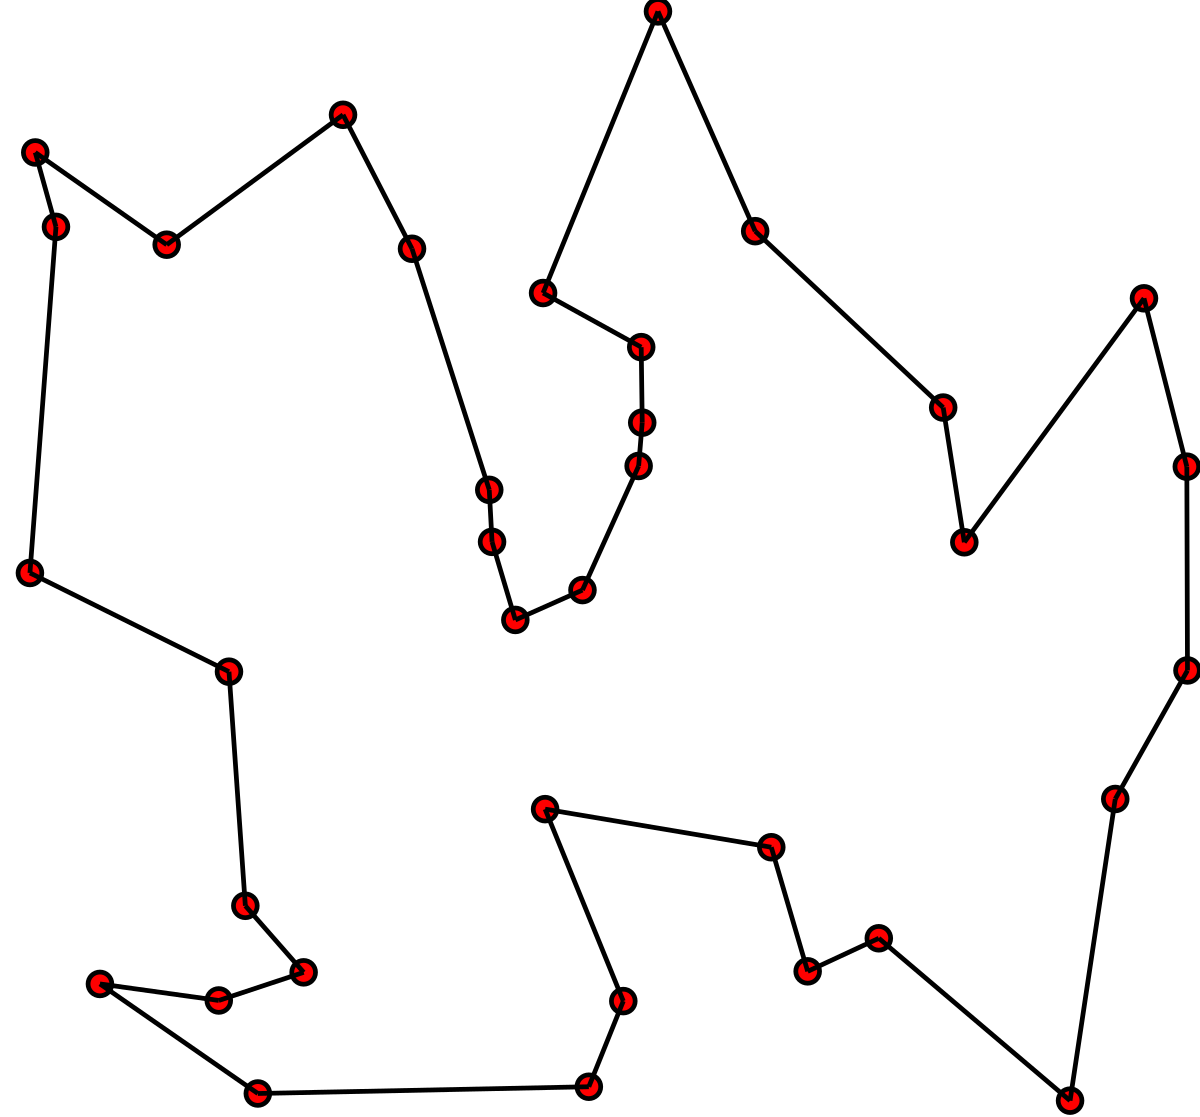
\includegraphics[scale=.15]{docs/pictures/tsp.png}
 \caption{TSP interpreted as a graph where a path is found. \cite{wiki:TSP}}
 \label{Figure:TSP-as-graph}
\end{figure}

\noindent
The travelling salesman problem could also be interpreted as a weighted undirected graph$_{\ref{undirected weighted graph}}$ with some number of nodes. Each node represents a city that the travelling salesman has to visit. The edges between each pair of nodes have a specific value or length, which signifies the Euclidean distance between that pair of cities. Given any $2$ cities, the distance from city A to city B is always the same as the distance from city B to city A.
\newline
Variations of the traveling salesman problem exist \cite{gutin_punnen_2007}, however, the version where the goal is to minimize the distance in Euclidean space is currently an NP-complete$_{\ref{NP-complete}}$ problem \cite{PAPADIMITRIOU1977}. 
\newline
Evidence shows that there exist no algorithms that could find the definite shortest path in polynomial time, at the same time as there are no algorithms that can guarantee any accuracy in any given map with cities. Other than that, verifying if any specific path is the most optimal is also unmanageable. \cite{PAPADIMITRIOU1977}
\newline
For example, a brute force solution could be considered to solve the classic travelling salesman problem, where all possible permutations of the order are computed, and then picking the shortest path out of all possible paths. Although this would be applicable to a smaller number of cities, the number of permutations possible would have a factorial$_{\ref{factorial}}$ growth the more cities that are required to be visited. 
\newline
It is an NP-hard problem and there are a lot of different heuristic$_{\ref{Heuristic}}$ algorithms. Some algorithms are more efficient in some situations than others. In this research, different algorithms are going to be tested on different test cases within a set amount of time. The algorithms being tested in this paper are a random generation algorithm, a modified Dijkstra's algorithm, a genetic algorithm with random swapping, and a genetic algorithm with 2-opt swapping.
\newline
The relevance and application of the travelling salesman problem in the real world such as optimizing routes for delivery vehicles, robots, or public transportations to minimize the travel distances, reduce fuel costs, and improve overall efficiency. The travelling salesman problem could also be applied to more technical concepts, such as finding the most optimal way to drill a circuit board or finding the most efficient order for sequencing genetic material such as DNA. 

\subsection{Aim}\label{Aim}
The aim of this paper is to find the limits of different heuristic algorithms for solving the travelling salesman problem. 

\subsection{Research Question}\label{RQ}
What algorithm out of the random generation algorithm, Dijkstra's algorithm, random swapping algorithm, and the 2-opt swapping are most efficient in finding the shortest path in a weighted graph, in a set amount of time?



\subsection{Theory}\label{Theory}

\subsubsection{Notations and definitions}\label{Notation and definitions}

This section explains a list of basic mathematical and computer scientific definitions and terms. 
\newline

\begin{enumerate}   %use the following to refer back to this part:
                    %$_{\ref{Polynomial}}$
 
  \item The \textbf{\textit{Euclidean distance}} between two points $p_1=(x_1,y_1)$ and $p_2=(x_2,y_2)$ is defined as $\sqrt{(x_2-x_1)^2+(y_2-y_1)^2}$. \label{Euclidean distance}
  \item An \textbf{\textit{undirected weighted graph}} is a type of graph where edges connect vertices, and each edge has an associated weight or cost. In an undirected graph, the edges do not have a specified direction, meaning they can be traversed in both directions.\label{undirected weighted graph}
  \item A problem is \textbf{\textit{NP-complete}} if no efficient algorithm is currently known that, could solve all instances of the problem in a reasonable amount of time. The term "complete" in NP-complete signifies that these problems are among the hardest problems in the class NP. If an efficient algorithm can be found for any NP-complete problem, it would imply that efficient algorithms exist for all problems in NP, which is considered highly unlikely. \label{NP-complete}
  \item The \textbf{\textit{factorial}} of a given non-negative integer $n$ is denoted by "$n!$". It is the product of all positive integers less than or equal to $n$. $$n! = n \cdot (n-1) \cdot (n-2) \cdot ... \cdot 2 \cdot 1 .$$ \label{factorial}
  \item The \textbf{\textit{triangle inequality}} states that for any three points A, B, and C in a space, the distance between A and C is always less than or equal to the sum of the distances between A and B, and between B and C. Another way to interpret the triangle inequality is by drawing a triangle, and observing how each side of the triangle will always be shorter or equal in length to the sum of the other $2$ sides. \label{Triangle Inequality}
  
    \begin{figure}[ht]
     \centering
     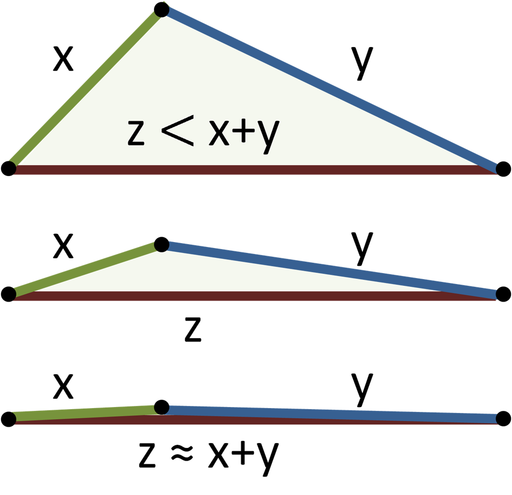
\includegraphics[scale=0.3]{docs/pictures/TriangleInequality.png}
     \caption{Examples of the triangle inequality for triangles with the side-lengths x, y, and z. \cite{wiki:Triangle}}
     \label{Figure:TriangleInequality}
    \end{figure}
    
\end{enumerate}




\subsubsection{Big O Notation}\label{Big O}
When computer scientists want to compare different kinds of algorithms, they can describe the efficiency of the algorithm with a mathematical function that describes the estimated run time of the algorithm using Big O notation. Big O notation is a way of describing the time complexity of an algorithm, which refers to how long an algorithm takes to complete based on the size of its input. The big O notation shows a huge difference when comparing the worst-case scenarios for each algorithm.
\newline
The "O" in Big O notation stands for "order of magnitude", which means that the function described grows a the same rate or within a constant factor as the function that is given. Hence when describing time complexities using big O notation, the coefficient becomes irrelevant. For example, an algorithm such as calculating the roots of a quadratic equation takes a constant time regardless of the size of the coefficients and has a time complexity of $O(1)$, even though the algorithm could possibly perform more than $1$ operation. If the time complexity of an algorithm grows linearly with the size of the input, the time complexity of the algorithm would be $O(n)$. An example of an algorithm with a linear time complexity would be to calculate the sum of an array with $n$ integers. The algorithm would be required to iterate through the whole array, as long as no other sum using this array has been pre-computed. Some other examples of common time complexities are: $O(\log{n})$, $O(n \log{n})$, $O(n^2)$, $O(2^n)$, and $O(n!)$.


\newline

\subsubsection{Heuristic Algorithms}\label{Heuristic}
When trying to solve a computational problem, it is crucial to find a relatively fast approach that is both efficient in finding the most optimal path and in a short period of time, especially when a large amount of input is considered. A common rule of thumb within competitive programming is to always use a program that performs less than $10^7$ operations.
\newline
As mentioned in the background, a brute force solution trying all possible paths for the travelling salesman problem would take an exceeding number of operations to compute. The time complexity of a brute force solution would be $O(n!)$, which means that it would be a sufficient enough algorithm if the number of cities would be less or equal to $10$, since $10! = 3628800 < 10^7$ and $11! > 10^7$. Any map with more than $10$ cities would take a lot more time before stopping to compute, while maps with more than $1000$ would not even stop computing after several years.
\newline
When the optimal solution is either unknown or computationally infeasible to find within a reasonable time frame, heuristic algorithms are used instead to provide an approximate solution. These algorithms prioritize efficiency and practicality over exact optimality. In this research, several different heuristic algorithms are used to repeatedly find the shortest path for the travelling salesman problem, and all the heuristic algorithms used will have a time complexity that is either $O(n)$ or $O(n \log{n})$. This also implies that maps with up to $10^6$ cities could be experimented on these algorithms without spending an unreasonable amount of time waiting for the algorithms to stop computing.
\newline
The heuristic algorithms compared to solve the travelling salesman problem in this research are:
\begin{itemize}
  \item Random generation algorithm.
  \item A modified version of Dijkstra's Algorithm.
  \item Self-improving Algorithm with Random Swapping.
  \item Self-improving Algorithm with 2-opt swapping.
\end{itemize}


\subsubsection{Random Generation Algorithm}\label{Random}
The random generation algorithm generates a random permutation of all possible nodes and calculates the length of the path generated. It always stores the path with the shortest path and repeats this algorithm until the time limit is reached. The algorithm is similar to repeatedly throwing some amount of dice, and after each throw the sum of all the results is stored. The more dice there are, the smaller the probability for the throw to result in the highest number possible.

\begin{algorithm}
\caption{Algorithm that generates random paths}\label{Random Algorithm}
\begin{algorithmic}

\While{Less than 2 seconds has passed}
\State $order \gets $ random permutation of the $n$ nodes
\State $currPath \gets calculatePath(order)$
\If{$bestPath > currPath$}
\State $bestOrder \gets order$
\State $bestPath \gets currPath$
\EndIf
\EndWhile

\end{algorithmic}
\end{algorithm}

\noindent
This algorithm has a time complexity of $O(n)$, since the generation of a random path has to iterate through each possible city. One assumption could be made for the random generation algorithm, which is that it is very unlikely for it to find the most optimal path when there are a lot of cities. Especially when no other optimization is applied to make the path shorter. However, for maps with less number of cities, it is likely for the algorithm to randomly find the best path within a reasonable time limit. Similarly, for any number of cities, as long as enough time is given for the algorithm, it would eventually find the shortest path. Nevertheless, in that case, where the algorithms could run for an infinite amount of time, the brute force solution would always guarantee finding the shortest solution.

\subsubsection{Modified Dijkstra's Algorithm}\label{Dijkstras}
Dijkstra's algorithm is an algorithm used on weighted, directed graph with non-negative weights. Dijkstra's algorithm will find the shortest path between a source node and all other nodes in a weighted graph. The algorithm maintains a priority queue of nodes and repeatedly selects the node with the smallest known distance from the source. It then updates the distances of its neighboring nodes, considering the weights of the edges. This process continues until all nodes have been visited, and the shortest path from the source to each node is determined. It can find a relatively short path within a reasonable time limit, but it is not guaranteed it will find the shortest path. In some way, Dijkstra's algorithm could be visualized as always picking the shortest path between two given nodes in the graph. Furthermore, the original Dijkstra's algorithm is used on a directed graph, starting from a source node and ending on any other node in the graph. However, that is not the case of the travelling salesman problem.
\noindent
A modified version of Dijkstra's algorithm could be applied to the travelling salesman problem instead. Given a starting node, iterate through all other unvisited nodes and find the shortest distance. This process is repeated on the node that had the shortest distance from the previous node until all nodes have been visited. 
\noindent
It might seem that this approach will always find the shortest path, however, there are cases where this approach does not do that. 

%show example of where dijkstra's algorithm doesn't work

Furthermore, this version of Dijkstra's algorithm's time complexity would be $O(n^2)$, since for each node, the distance to all other nodes has to be calculated. 



originally a $O(n^2)$ algorithm. however, by only comparing the log2(n) random neighbors, it would become $O(nlog(n))$

\subsubsection{Self-improving Algorithm with Random Swapping}\label{Random Swapping}
algorithm that requires $O(n)$. however for each swap, it takes $O(1)$. run until 2 seconds has gone by.

Similar to natural selection.

This algorithm starts off with a randomly generated path. After that, two nodes are randomly chosen. Using the current neighbors of those nodes it is possible to calculate the change in the length distance, if the nodes were swapped. If this creates a longer path than before, then the nodes are not swapped. However, if the change would make the path shorter, then the nodes are swapped.



\subsubsection{Self-improving Algorithm with 2-opt swapping}\label{2-opt swapping}
algorithm that requires $O(n)$. however for each swap, it takes $O(1)$. run until 2 seconds has gone by.

Similar to the self-imporving algorithm with random swapping, this algorithm also starts off wiht a randomly generated path. Then two random edges are randomly chosen and swapped. 

Triangle inequality?
have pictures showing that two edges that cross each other are bad.

\subsubsection{Maps}\label{maps}
How does each map get generated?

map4 Sweden: \href{https://github.com/sphrak/svenska-stader/blob/master/src/svenska-stader.csv}{github}  took the top 1000 or 10000 most populated cities in sweden

map5: \href{https://developers.google.com/public-data/docs/canonical/states_csv}{dev google}

49 cities, without Hawaii, Alaska and Puerto Rico.


\subsubsection{Integers vs floats}\label{Int vs Float}
Integers and floats are two common data types for numbers. Integers are used to store whole numbers, while floats are used to store decimal numerals. Computers are known to be very inefficient when it comes to handling float numbers.
this is why all coordinates of the maps are integers, even though coordinates on a real map are not necessarily integers. 




\section{Method}\label{Method}
Firstly, $10$ different maps with various numbers of cities were generated$_{\ref{maps}}$. The $10$ different maps with test data were run on $4$ separate algorithms that are made to solve the traveling salesman problem using Euclidean distance. The algorithms used were: Random generation algorithm$_{\ref{Random}}$, Modified Dijkstra's algorithm$_{\ref{Dijkstras}}$, self-improving algorithm with random swapping$_{\ref{Random Swapping}}$, and self-improving algorithm with 2-opt swapping$_{\ref{2-opt swapping}}$. All algorithms were written in Python 3, and all tests were run on Python version 3.10.6 64-bit. Each map was tested with each algorithm $6$ times, which means that there were $6$ replicates of each combination of map and algorithm. Several replicates were made since randomness since a factor of randomness is involved in each algorithm. For each execution of the algorithm, a time limit was a maximum of 2 seconds. After all runs, the paths found were recorded as well as the length of the path. The results can be compared across different maps, and if possible, a correlation could be found. 
\noindent
The constant variables of this method are the various maps, the time limit, and the programming language used, which was Python 3. The independent variable is the algorithm used for each replicate, and the dependent variable is the length of the shortest path found using these algorithms.


\subsection{Limitations}\label{Limitations}
One limitation is the scope of algorithms used. This study only considers $4$ algorithms for solving the travelling salesman problem. However, there could be other algorithms that are not included in the study that could perform better in a similar time-constrained environment. Similarly, combinations of these algorithms are also possible to create and could in the same way also be a more optimal option than the algorithms used. 
\noindent
At the same time, the algorithms used in the study may require more fine-tuning on various parameters to achieve even more optimal performance. 
\noindent
Another limitation is the different maps used. Since only $10$ different maps are being considered here, it would not represent fully all possible scenarios. This should be taken into consideration before drawing any generalized conclusion from the results of these maps.


\section{Results}\label{Results}

Explain that the results are given in units of length. 
Also make the best result on each map bold, and calculate the average for each algorithm on each map.





\begin{table}[H]
    \centering
    \begin{tabular}{|p{0.2\linewidth}|p{0.2\linewidth}|p{0.2\linewidth}|p{0.2\linewidth}|}
    \hline
        \textbf{Map 1 } & random n=10 & ~ & ~ \\ \hline
        \textbf{Random Generation} & \textbf{Modified Dijkstra's} & \textbf{Random Swapping} & \textbf{2-opt swapping} \\ \hline
        5891573.876 & 5891573.876 & 5891573.876 & 5891573.876 \\ \hline
        5891573.876 & 5891573.876 & 5891573.876 & 5891573.876 \\ \hline
        5891573.876 & 5891573.876 & 5891573.876 & 5891573.876 \\ \hline
        5891573.876 & 5891573.876 & 5891573.876 & 5891573.876 \\ \hline
        5891573.876 & 5891573.876 & 5891573.876 & 5891573.876 \\ \hline
        6131798.7 & 5891573.876 & 5891573.876 & 5891573.876 \\ \hline
    \end{tabular}
\end{table}

\begin{table}[H]
    \centering
    \begin{tabular}{|p{0.2\linewidth}|p{0.2\linewidth}|p{0.2\linewidth}|p{0.2\linewidth}|}
    \hline
        \textbf{Map 2 (random n=1000)} & ~ & ~ & ~ \\ \hline
        \textbf{Random Generation} & \textbf{Modified Dijkstra's} & \textbf{Random Swapping} & \textbf{2-opt swapping} \\ \hline
        992924716.9 & 375916823.6 & 225977937.9 & 72516889.45 \\ \hline
        987691105 & 372737685.5 & 229849151.6 & 69427895.87 \\ \hline
        995151465.5 & 369072515.4 & 221449499.6 & 68808723.25 \\ \hline
        989088278.2 & 371810727.2 & 232695937.3 & 69720673.41 \\ \hline
        989255767.2 & 373373480 & 233207053.9 & 70331677.81 \\ \hline
        991826128.7 & 373281345.9 & 207510610.3 & 69670533.67 \\ \hline
    \end{tabular}
\end{table}

\begin{table}[H]
    \centering
    \begin{tabular}{|p{0.2\linewidth}|p{0.2\linewidth}|p{0.2\linewidth}|p{0.2\linewidth}|}
    \hline
        \textbf{Map 3 (random n=10000)} & ~ & ~ & ~ \\ \hline
        \textbf{Random Generation} & \textbf{Modified Dijkstra's} & \textbf{Random Swapping} & \textbf{2-opt swapping} \\ \hline
        10323119546 & 3240428284 & 3793530293 & 3152792905 \\ \hline
        10279776945 & 3233877905 & 3776841645 & 2937278015 \\ \hline
        10298645329 & 3234864733 & 3822141990 & 3095200214 \\ \hline
        10298914814 & 3234688577 & 3842225040 & 3020962352 \\ \hline
        10285436723 & 3228157454 & 3828077792 & 2984305232 \\ \hline
        10300080362 & 3232665916 & 3807533962 & 3049464688 \\ \hline
    \end{tabular}
\end{table}

\begin{table}[H]
    \centering
    \begin{tabular}{|p{0.2\linewidth}|p{0.2\linewidth}|p{0.2\linewidth}|p{0.2\linewidth}|}
    \hline
        \textbf{Map 4 (Swedish cities n=1916)} & ~ & ~ & ~ \\ \hline
        \textbf{Random Generation} & \textbf{Modified Dijkstra's} & \textbf{Random Swapping} & \textbf{2-opt swapping} \\ \hline
        79693630.34 & 27564839.82 & 20262321.82 & 6084857.948 \\ \hline
        79693630.34 & 27473123.85 & 19561130.69 & 6204447.677 \\ \hline
        79693630.34 & 27566245.04 & 19480924.3 & 5934914.712 \\ \hline
        79693630.34 & 27734229.92 & 19246108.98 & 5871981.884 \\ \hline
        79693630.34 & 27636185.38 & 20044024.37 & 5924928.645 \\ \hline
        79693630.34 & 27755956.26 & 19643845.39 & 6129804.537 \\ \hline
    \end{tabular}
\end{table}

\begin{table}[H]
    \centering
    \begin{tabular}{|p{0.2\linewidth}|p{0.2\linewidth}|p{0.2\linewidth}|p{0.2\linewidth}|}
    \hline
        \textbf{Map 5 (USA states n=49)} & ~ & ~ & ~ \\ \hline
        \textbf{Random Generation} & \textbf{Modified Dijkstra's} & \textbf{Random Swapping} & \textbf{2-opt swapping} \\ \hline
        63470.66185 & 32761.02342 & 23363.90715 & 18288.09154 \\ \hline
        63890.85113 & 31608.6966 & 23739.19883 & 18205.1266 \\ \hline
        64490.2589 & 31536.60587 & 21482.12635 & 18234.21287 \\ \hline
        62379.14452 & 31131.14313 & 22779.03298 & 18311.86805 \\ \hline
        66385.01545 & 31806.5271 & 23763.20389 & 18311.86805 \\ \hline
        60399.75765 & 31211.23317 & 20760.25464 & 18300.61299 \\ \hline
     \end{tabular}
\end{table}

\begin{table}[H]
    \centering
    \begin{tabular}{|p{0.2\linewidth}|p{0.2\linewidth}|p{0.2\linewidth}|p{0.2\linewidth}|}
    \hline
        \textbf{Map 6 (Strict increase n=10000)} & ~ & ~ & ~ \\ \hline
        \textbf{Random Generation} & \textbf{Modified Dijkstra's} & \textbf{Random Swapping} & \textbf{2-opt swapping} \\ \hline
        9291380109 & 1349024996 & 2373586959 & 1814447149 \\ \hline
        9310437819 & 1348572833 & 2280159165 & 1455553611 \\ \hline
        9297883462 & 1357296776 & 2344747004 & 1601361008 \\ \hline
        9302381835 & 1353080817 & 2306799937 & 1599620455 \\ \hline
        9286799450 & 1350374546 & 2325432171 & 1593378825 \\ \hline
        9329019143 & 1348033186 & 2361945269 & 1646813150 \\ \hline
    \end{tabular}
\end{table}

\begin{table}[H]
    \centering
    \begin{tabular}{|p{0.2\linewidth}|p{0.2\linewidth}|p{0.2\linewidth}|p{0.2\linewidth}|}
    \hline
        \textbf{Map 7 (Circle n=10000)} & ~ & ~ & ~ \\ \hline
        \textbf{Random Generation} & \textbf{Modified Dijkstra's} & \textbf{Random Swapping} & \textbf{2-opt swapping} \\ \hline
        12567650338 & 2248980912 & 3908157889 & 2537013830 \\ \hline
        12573745599 & 2217757665 & 3952339027 & 2431780351 \\ \hline
        12600808851 & 2244295348 & 3929417131 & 2620719310 \\ \hline
        12577611347 & 2237577332 & 3851583858 & 2445124971 \\ \hline
        12549889305 & 2238673128 & 3951409612 & 2557729463 \\ \hline
        12551595182 & 2245565916 & 3884563307 & 2602087504 \\ \hline
    \end{tabular}
\end{table}

\begin{table}[H]
    \centering
    \begin{tabular}{|p{0.2\linewidth}|p{0.2\linewidth}|p{0.2\linewidth}|p{0.2\linewidth}|}
    \hline
        \textbf{Map 8 (Grid n=10000)} & ~ & ~ & ~ \\ \hline
        \textbf{Random Generation} & \textbf{Modified Dijkstra's} & \textbf{Random Swapping} & \textbf{2-opt swapping} \\ \hline
        516272.1618 & 162933.9379 & 189487.4362 & 146595.3781 \\ \hline
        515198.6725 & 162480.318 & 185568.5141 & 148485.5344 \\ \hline
        515030.9863 & 162150.3042 & 186938.2779 & 148197.8332 \\ \hline
        516285.3527 & 162161.47 & 186978.8585 & 148080.8074 \\ \hline
        513969.2742 & 161665.9353 & 184770.9426 & 142505.3975 \\ \hline
        514867.3062 & 162288.9124 & 186445.5991 & 148529.9744 \\ \hline
    \end{tabular}
\end{table}

\begin{table}[H]
    \centering
    \begin{tabular}{|p{0.2\linewidth}|p{0.2\linewidth}|p{0.2\linewidth}|p{0.2\linewidth}|}
    \hline
        \textbf{Map 9 (Straight line n=10000)} & ~ & ~ & ~ \\ \hline
        \textbf{Random Generation} & \textbf{Modified Dijkstra's} & \textbf{Random Swapping} & \textbf{2-opt swapping} \\ \hline
        6553370088 & 949184378 & 1656974798 & 896028426 \\ \hline
        6565113386 & 946308942 & 1643517954 & 903780140 \\ \hline
        6506833168 & 961167540 & 1620169650 & 808419124 \\ \hline
        6545958006 & 945003364 & 1668749822 & 787330814 \\ \hline
        6535809660 & 956124694 & 1613793366 & 806036378 \\ \hline
        6562710126 & 951048114 & 1582440390 & 779322396 \\ \hline
    \end{tabular}
\end{table}

\begin{table}[H]
    \centering
    \begin{tabular}{|p{0.2\linewidth}|p{0.2\linewidth}|p{0.2\linewidth}|p{0.2\linewidth}|}
    \hline
        \textbf{Map 10 (Strict increase n=100)} & ~ & ~ & ~ \\ \hline
        \textbf{Random Generation} & \textbf{Modified Dijkstra's} & \textbf{Random Swapping} & \textbf{2-opt swapping} \\ \hline
        67609575.19 & 20823427.49 & 11069509.51 & 5815136.523 \\ \hline
        69664811.6 & 20805907.35 & 11533087.55 & 5810589.705 \\ \hline
        67715528.88 & 20874288.9 & 10755444.78 & 5804089.746 \\ \hline
        68228851.14 & 21454217.01 & 12453953 & 5792401.336 \\ \hline
        68862987.39 & 19999070.68 & 12382933.57 & 5812265.15 \\ \hline
        70379810.37 & 21192230.7 & 10883480.63 & 5800222.75 \\ \hline
    \end{tabular}
\end{table}



\newpage


\section{Discussion}\label{sec4}

\subsection{Generalized Results}\label{subsec1}
which algorithm showed the best results overall?

First of all, when the number of cities is small enough, all cities will find the shortest path possible given 2 seconds of running as shown in the results of map 1. This could be explained since there are $n!$ permutations in total, and if $n\leq 10$, the algorithms could in theory calculate and find the shortest path within the time limit.

Random generation performed the worst out of all of these four algorithms, which could be explained since no kind of optimization to find the shortest path is utilized when generating the random path. 

Between the two self-improving algorithms, the 2-opt swapping performed better compared to random swapping across all the maps tested in this experiment. 

\subsection{Specified Results }\label{subsec2}
what algorithm could be good in what situation?

Modified Dijkstra's algorithm works best out of these four when there is a clear path across the map and when there are a high number of nodes close to each other that are the closest. Some examples of the maps the modified Dijkstra's algorithm excels at are map 6 and map 7. 

2-opt is generally good, but especially on maps where it is common that crosses exist. Since 2-opt will generally make changes if the two chosen edges cross each other since swapping them would lead to a shorter path.


\subsection{Evaluation and further research}\label{subsec3}

further research should be conducted with:
using $O(n^2)$ algorithms such as 
greedy algorithm
Christofides algorithm - guarantees to be within a factor of 3/2 of the optimal solution length \cite{Christofides}
Simulated annealing.
3 opt. or even Lin-Kernighan Heuristic algorithm
Longer time-constraints?
combination of these? For example start with a greedy solution, and then improve it by applying 3-opt.
more maps with differnet shapes and distributions should be used.

\section{Conclusion}\label{sec5}






\newpage
\bibliographystyle{apacite}
\bibliography{references.bib} \label{sec6}



\end{document}
